%%%%%%%%                        01 - Motivace                       %%%%%%%%
%---------------------------------------------------------------------------
% Při prezentování nejvíc záleží na začátku. 
% Pro získání pozornosti na začátku veřejné řeči se doporučuje: říct nějakou statistiku; položit otázku (u státnic spíše řečnickou).

% HEROUT, Adam. Prezentování. Herout.net: Poznámky učitele, kouče, čtenáře. [online]. [cit. 2021-9-15]. Dostupné z: https://www.herout.net/blog/category/prezentovani/
%---------------------------------------------------------------------------

% - Uveďte posluchače do tématu své práce.
% - Řekněte něco málo o stavu před zahájením práce a jaké byly důvody pro její vypracování.
% - Nejlepší je vysvětlit motivaci pomocí schématu. Pokud musíte použít odrážky, tak super-stručné, abyste je nečetli, ale ony pouze tvořily kostru sdělení.

% Z této části prezentace musí posluchači dostat stručné a výstižné odpovědi na otázky:
%  A) Proč děláte, co děláte? K čemu je to dobré?
%  B) Co je cílem práce? Co má být výsledkem?

% Odolejte pokušení říkat banality a všeobecně známé informace.
% "Žijeme v době rozvoje mobilní výpočetní techniky, kdy každý má v kapse mobil" - je dokonale prázdné a hloupé sdělení, nic takového neříkejte, fakt to nikoho nezajímá.

\begin{frame}
  \frametitle{Úvod do problematiky}
  \begin{columns}
    \column{0.4\textwidth}
    \begin{itemize}
        \phantom{\item Nedostatky stávajících řešení}
        \phantom{\item Neexistence univerzálního řešení}
        \phantom{\item Neexistence triviálně použitelného řešení}
    \end{itemize}
     
    \column{0.6\textwidth}
    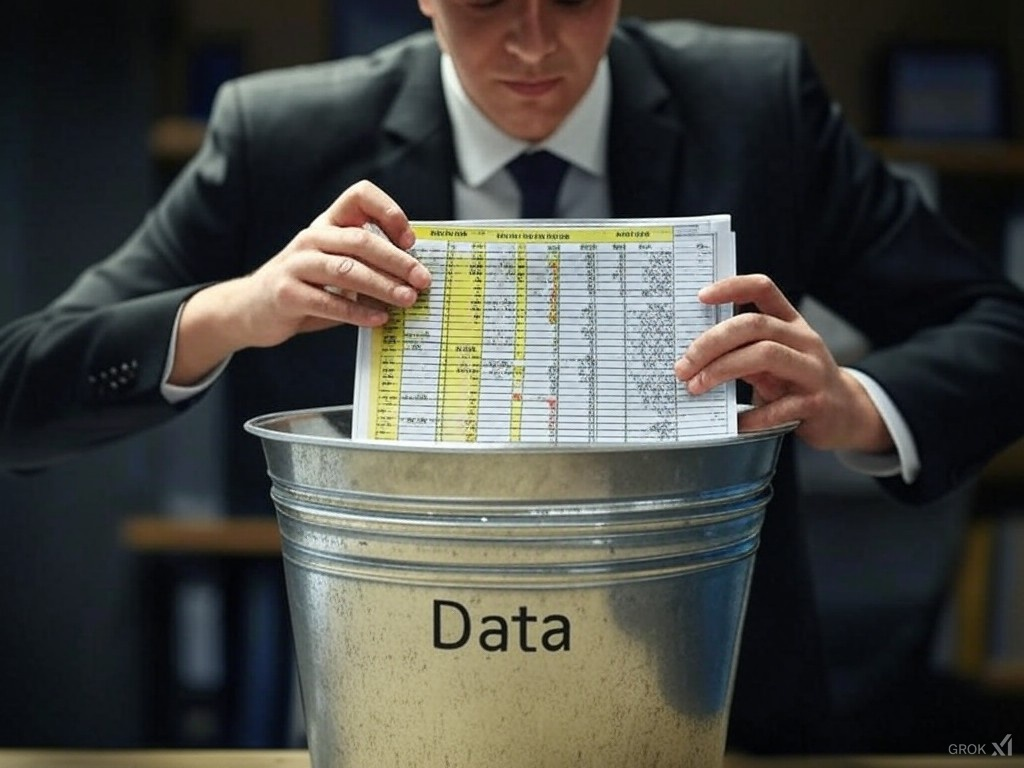
\includegraphics[width=\textwidth]{img/data-bucket.jpg}
  \end{columns}
\end{frame}

\begin{frame}
  \frametitle{Motivace}
  \begin{columns}
    \column{0.4\textwidth}
    \begin{itemize}
        \item \emph{Nedostatky stávajících řešení}
        \phantom{\item Neexistence univerzálního řešení}
        \phantom{\item Neexistence triviálně použitelného řešení}
    \end{itemize}
     
    \column{0.6\textwidth}
    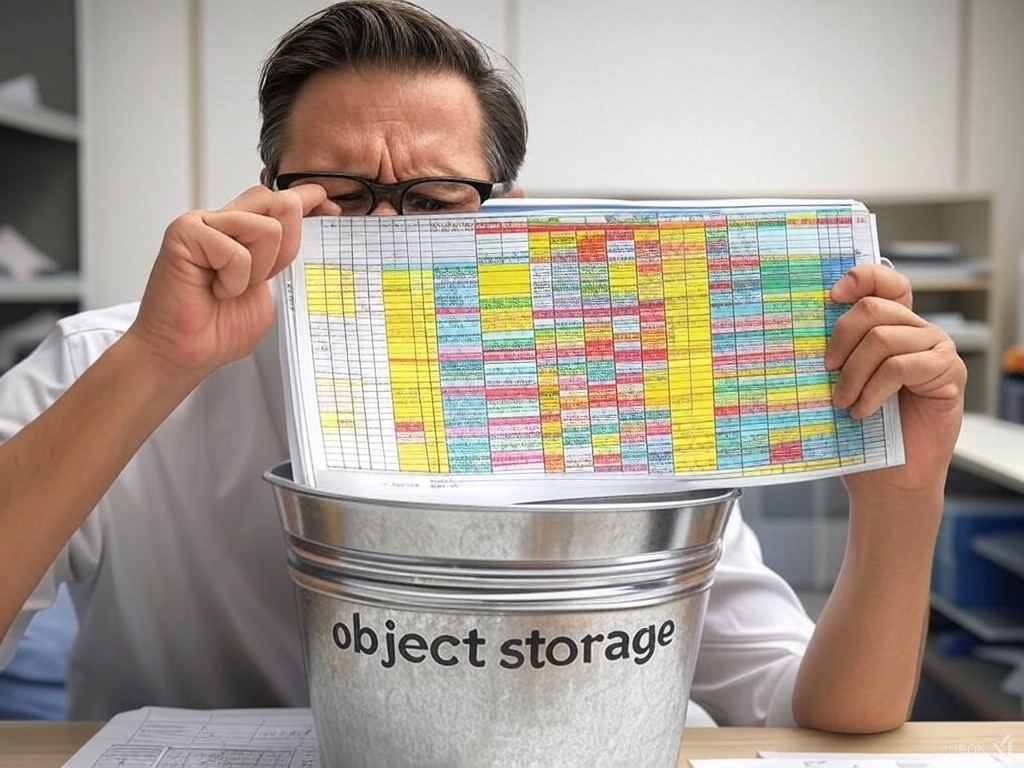
\includegraphics[width=\textwidth]{img/spreadsheet-doesnt-fit.jpg}
  \end{columns}
\end{frame}

\begin{frame}
  \frametitle{Motivace}
  \begin{columns}
    \column{0.4\textwidth}
    \begin{itemize}
        \item Nedostatky stávajících řešení
        \item \emph{Neexistence univerzálního řešení}
        \phantom{\item Neexistence triviálně použitelného řešení}
    \end{itemize}
     
    \column{0.6\textwidth}
    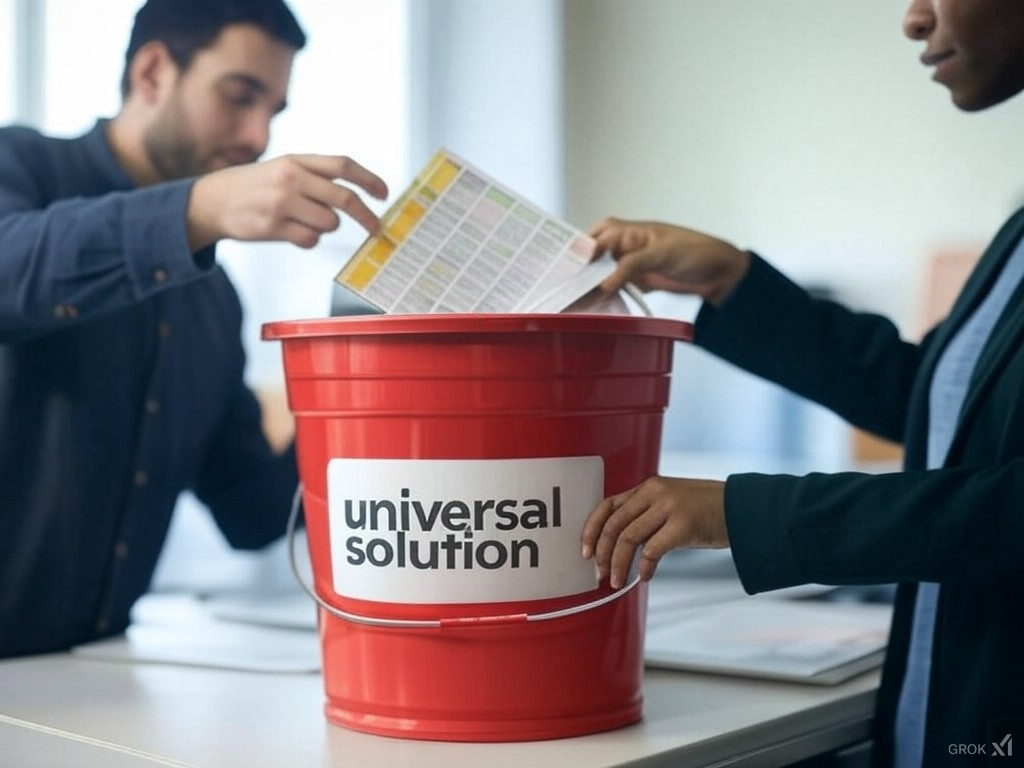
\includegraphics[width=\textwidth]{img/universal-solution.jpg}
  \end{columns}
\end{frame}

\begin{frame}
  \frametitle{Motivace}
  \begin{columns}
    \column{0.4\textwidth}
    \begin{itemize}
        \item Nedostatky stávajících řešení
        \item Neexistence univerzálního řešení
        \item \emph{Neexistence triviálně použitelného řešení}
    \end{itemize}
     
    \column{0.6\textwidth}
    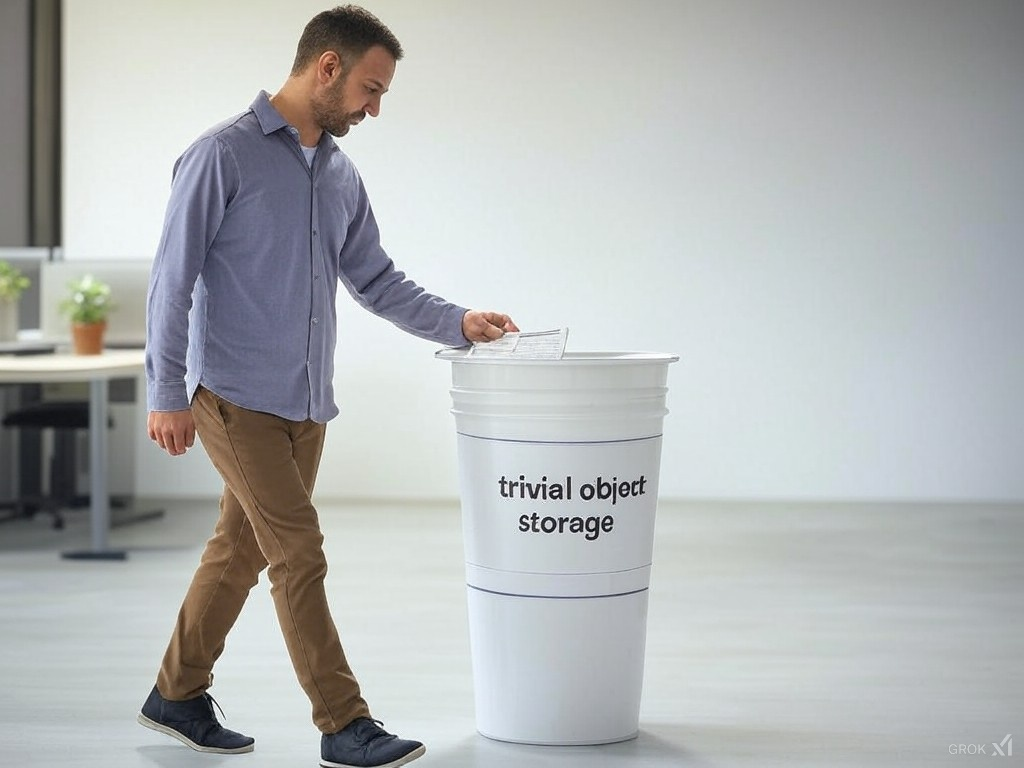
\includegraphics[width=\textwidth]{img/trivial-solution-2.jpg}
  \end{columns}
\end{frame}


%%%%%%%%                       02 - Cíle práce                      %%%%%%%%
%---------------------------------------------------------------------------
% Stručně uveďte cíle Vaší práce.
% Vhodné jsou max. 3 odrážky/věty s hlavními cíli.

% Někdy je motivace totožná s formulací cílů. Nenuťte se do dvou slajdů, když je správnější myšlenku vyjádřit jedním... 

% Formulujte, co je cílem:
%  - Jak se pozná úspěšný výsledek?
%  - Co jsou výstupy?
%  - Jaké vlastnosti má mít úspěšný výsledek?
%  - Kde to půjde použít?

% Lepší je bez použití odrážek:
%  - mít dostatečně dobrý obrázek, který budete svými slovy komentovat 
%  - na obrázku je vizuální sdělení, sdělení slovní dodáte pusou

% Je zbytečné říkat generická a obecná tvrzení: "Řešení by mělo být rychlé, spolehlivé a robustní" - toto jsou obecné požadavky na cokoli a informační hodnota sdělení je NULA - je to jen plýtvání časem a inteligencí.
% Mluvte konkrétně: Jaké konkrétní vlastnosti má mít Vaše řešení, co konkrétně znamená "robustní", co konkrétně znamená "spolehlivé"?

\begin{frame}
  \frametitle{Cíl práce}
  \begin{columns}
    \column{0.4\textwidth}
    Vytvořit řešení, které je
    \begin{itemize}
        \item Triviální
        \item Univerzální
        \item Bezpečné
    \end{itemize}
     
    \column{0.6\textwidth}
        
\includegraphics[width=\textwidth]{img/universal-object-storage-3.jpg}
  \end{columns}
\end{frame}


%%%%%%%%                  03 - Informace o řešení                   %%%%%%%%
%---------------------------------------------------------------------------
% Cílem  obhajoby je podat zprávu o stavu projektu, nikoliv tedy držet přednášku na zadané téma. Mluvte o tom, co vy jste udělali, jaké jsou vaše výsledky. Mějte na slajdech formální pojmy, buďte přesní, definujte a odkazujte se.

% Prezentace nemusí a vlastně nemá obsahovat:
% -- Výklad použitých algoritmů apod. To patří do přednášky na dané téma, v prezentaci o stavu jen známé algoritmy uveďte podle jména, neznámé algoritmy třeba trochu přibližte, aby bylo zřejmo, o co jde, ale nevysvětlujte je podrobně. Není cílem, aby vaši posluchači algoritmu rozuměli a dokázali ho naprogramovat, ale aby měli představu, na čem pracujete a jak se vám to daří.
% -- Podrobnosti návrhu vašeho systému. Opět, posluchači nebudou váš systém hackovat, nepotřebují detailní strukturu tříd, názvy funkcí, jména souborů, datové formáty apod. Tyto věci uvádějte pouze v takové míře, která pomůže posluchačům udělat si představu, na čem pracujete a jak se vám to daří.

% HEROUT, Adam. Prezentování. Herout.net: Poznámky učitele, kouče, čtenáře. [online]. [cit. 2021-9-15]. Dostupné z: https://www.herout.net/blog/category/prezentovani/
%---------------------------------------------------------------------------

% - Uveďte, jaké zajímavé problémy jste v práci řešili.
% - Mělo by z toho být patrné, že je to závěrečná práce -- ne jen další projekt do předmětu -- tedy je v tom něco netriviálního, zajímavého a přínosného.
% - Raději dva nebo tři slajdy, které ukážete/vysvětlíte během 20 vteřin, než se snažit všechno "namastit" na jeden slajd.
% - Na slajdy je dobré dát vizuální informaci: vzorce, schemata, obrázky, diagramy. Slovní informaci můžete předat pusou. Je dokonale zbytečné a otravné mít na slajdu v odrážkách to samé, co se chystáte říct.
% - Titulek slajdu "Podstatné informace o řešení" je hodně generický. Ve skutečné Vaší prezentaci bude daleko lepší použít specifický titulek na každém ze slajdů, například: "Schéma neuronové sítě pro detekci frňáků", "Návrh nekonečného automatu", "Vytvořená datová sada" apod.

\iffalse
digraph DataProcessing {
    rankdir=LR;
    ratio=0.3;
    size="10";  // Sets max drawing size
    nodesep=0.3; // Space between nodes horizontally
    ranksep=0.5; // Space between ranks vertically
    node [shape=box, fontsize=10];
    Data [label="Data"];
    HashedData [label="hash(Data)"];
    DataChunk [label="DataChunk"];
    EncryptedDataChunk [label="EncryptedDataChunk"];
    HashOfEncrypted [label="Hash"];
    HKey [label="HKey"];

    Data -> DataChunk
    Data -> HashedData [label="hash"];
    Data -> Length [label=".len()"]
    {HashedData; "Length"} -> DataChunk [label="append"];
    DataChunk -> Key [label="hash"];
    DataChunk -> EncryptedDataChunk [label="encrypt"];
    Key -> EncryptedDataChunk [label="encryption key"];
    EncryptedDataChunk -> HashOfEncrypted [label="hash"];
    {HashOfEncrypted; Key} -> HKey [label="combine"];
}
\fi

\begin{frame}
  \frametitle{Formát serializace a způsob adresace dat}
  \makebox[\linewidth]{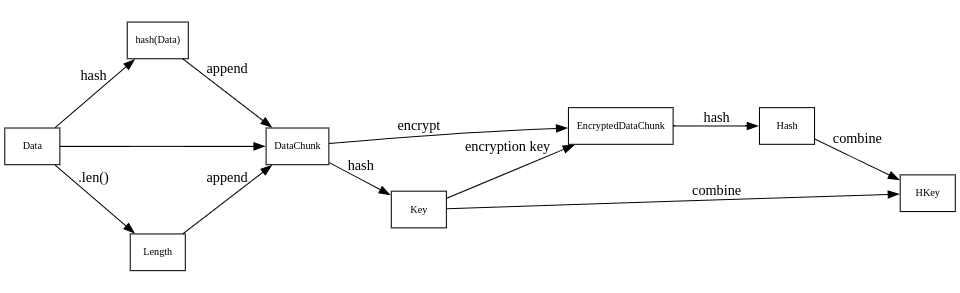
\includegraphics[width=\paperwidth]{img/hkey.png}}
\end{frame}

\iffalse
digraph G {
    rankdir=LR; // Make the graph horizontal
    node [shape=diamond, style=filled, fillcolor=lightblue]; // Diamond-shaped nodes

    // User application sends the chunk to the first node
    user [shape=box, style=filled, fillcolor=lightgrey, label="User Application"];
    user -> "KgNFe5fE" [label="sends AABBCCDD"];
    
    // The first node sends the chunk to other nodes
    "KgNFe5fE" -> "AABBCg5e" [label="sends AABBCCDD"];
    "KgNFe5fE" -> "AABBf5Ef" [label="sends AABBCCDD"];
    "KgNFe5fE" -> "AABCfEge" [label="sends AABBCCDD"];
}
\fi

\begin{frame}
  \frametitle{Metoda propagace dat}
  \makebox[\linewidth]{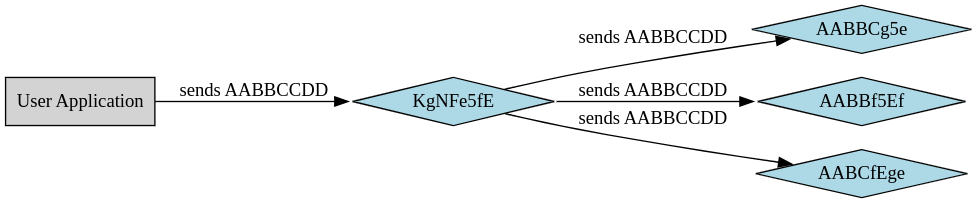
\includegraphics[width=\paperwidth]{img/sharing.png}}
\end{frame}

\iffalse
digraph G {
    rankdir=LR; // Make the graph horizontal
    node [shape=diamond, style=filled, fillcolor=lightblue]; // Diamond-shaped nodes

    // User application sends the chunk to the first node
    user [shape=box, style=filled, fillcolor=lightgrey, label="User Application 2"];
    user -> "jf9e4F4e" [label="requests AABBCCDD"];
    
    // The first node retreives the chunk from its peers
    "jf9e4F4e" -> "AABBCCDf" [label="requests AABBCCDD"];
    "AABBCCDf" -> "jf9e4F4e" [label="not found"];
    "jf9e4F4e" -> "AABBCg5e" [label="requests AABBCCDD"];
    "AABBCg5e" -> "jf9e4F4e" [label="sends AABBCCDD"];
    
    // finally, the chunk is send back to the user application
    "jf9e4F4e" -> user [label="sends AABBCCDD"];
}
\fi

\begin{frame}
  \frametitle{Metoda nalezení dat}
  \makebox[\linewidth]{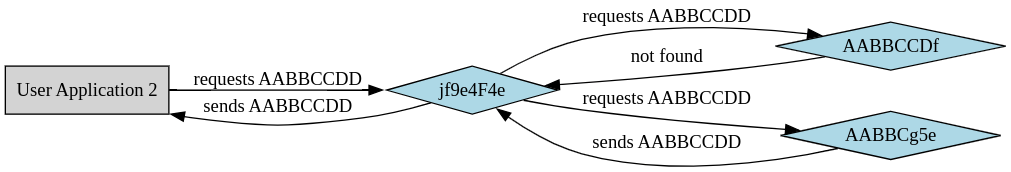
\includegraphics[width=\paperwidth]{img/seeking.png}}
\end{frame}

\begin{frame}
  \frametitle{Sdílení dat mezi aplikacemi}
  \makebox[\linewidth]{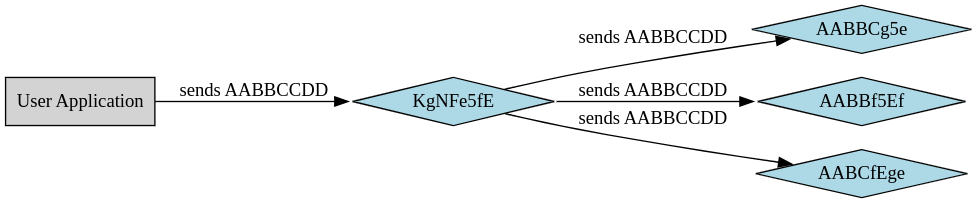
\includegraphics[width=\paperwidth]{img/sharing.png}}
  \makebox[\linewidth]{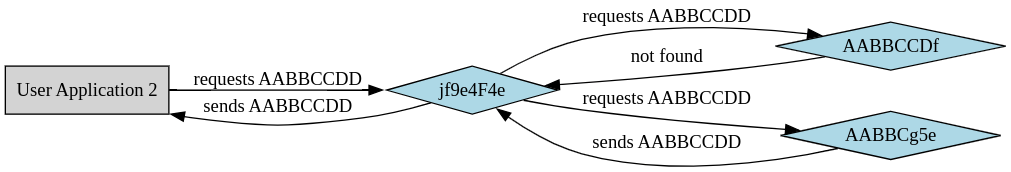
\includegraphics[width=\paperwidth]{img/seeking.png}}
\end{frame}

%%%%%%%%                    04 - Výsledky práce                     %%%%%%%%
%---------------------------------------------------------------------------
% Shrňte, jakých výsledků se Vám podařilo dosáhnout.
% Uveďte, jakým způsobem byla vyhodnocena funkčnost a správnost řešení.
% Buďte konkrétní: místo "Aplikace je otestovaná", řekněte, kým a jak byla testována, jaké byly výsledky testů.
% Místo "Úspěšnost detektoru je hodně dobrá" řekněte "Úspěšnost detektoru je 93 % mAP" nebo ještě radši ukažte tabulku se srovnáním oproti alternativním řešením.
% Pokud vyhodnocení sestávalo ze dvou nebo tří částí, může být vhodné rozdělit obsah na dva či tři slajdy. Při prezentování je ovšem potřeba se pohlídat, aby čas věnovaný každému slajdu byl adekvátně krátký a nedošlo k přetažení času.

\begin{frame}
  \frametitle{Stav práce}
  \textbf{Co je hotové:}
  \begin{itemize}
    \item Šifrovací modul \texttt{ps-cypher}
    \item Serializační modul \texttt{ps-datachunk}
    \item Úložný modul \texttt{ps-datalake}
    \item Knihovna generických procedur \texttt{ps-hkey}
  \end{itemize}
  \vspace{1em}
  \textbf{Co zbývá dokončit:}
  \begin{itemize}
    \item Komunikační modul \texttt{ps-datanode}
    \item Technická zpráva
  \end{itemize}
\end{frame}


%%%%%%%%                      05 - Poděkování                       %%%%%%%%
%---------------------------------------------------------------------------
% Na tomto slajdu by měl být buď jeden velký, nebo více menších vhodně poskládaných obrázků.
% Vyberte to nejlepší, čím se chcete pochlubit - komise se na tento slajd bude dívat nejdéle ze všech slajdů.
% U tohoto slajdu ústně poděkujete za pozornost (ne nutně textem přes celý slajd) a komise pak bude mít prostor pro jeho prohlížení při čtení posudků.
%---------------------------------------------------------------------------

% Co padne na konci prezentace, je to, co posluchači budou brát v úvahu při následném rozhodování.

% HEROUT, Adam. Prezentování. Herout.net: Poznámky učitele, kouče, čtenáře. [online]. [cit. 2021-9-15]. Dostupné z: https://www.herout.net/blog/category/prezentovani/
%---------------------------------------------------------------------------

\begin{frame}
  \frametitle{Děkuji za pozornost!}
  \makebox[\linewidth]{
\includegraphics[width=\paperwidth]{img/dotazy.png}}
\end{frame}
